\subsubsection{First touch}
Les résultats de la factorisation et de la résolution triangulaire avec une allocation first touch sur la machine  sont exposés dans le chapitre précèdent.
%
Les résultats ne sont pas aussi bons que ceux que nous pourrions obtenir avec une meilleure gestion de la mémoire.
%
Pour rappel, nous obtenions au mieux une accélération de 8,7 sur coeurs pour la factorisation et une accélération de 2,8 pour la résolution triangulaire.


Sur la machine Manumanu, nous obtenons le même type d'accélération que pour le SpMV.
%
Tant que nous utilisons moins de 2 bancs NUMA, nous obtenons une accélération de 10 pour la factorisation (Fig.~\ref{fig:res_facto_ft_manumanu}) et une accélération de 6,2 pour la résolution triangulaire (Fig.~\ref{fig:res_trsv_ft_manumanu}).


%   (-_-)   %
\begin{figure}[!ht]
     \begin{center}
        \subfigure[Factorisation ILU(0).]{%
          \label{fig:res_facto_ft_manumanu}
          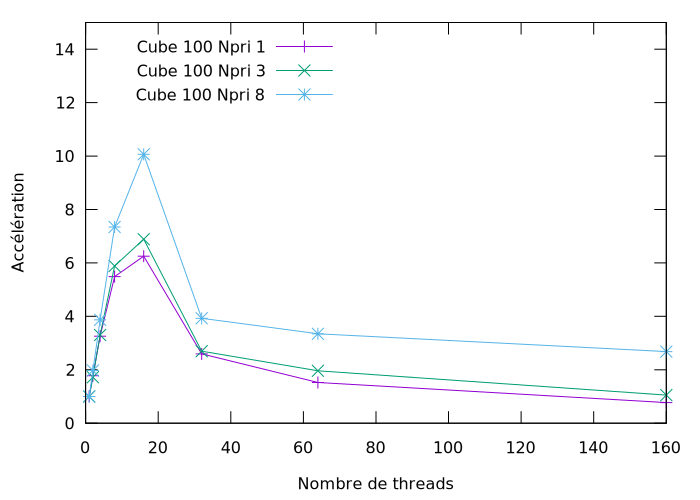
\includegraphics[width=0.49\textwidth]{res_facto_ft_manu}
        }%
        \subfigure[Résolution triangulaire]{%
          \label{fig:res_trsv_ft_manumanu}
          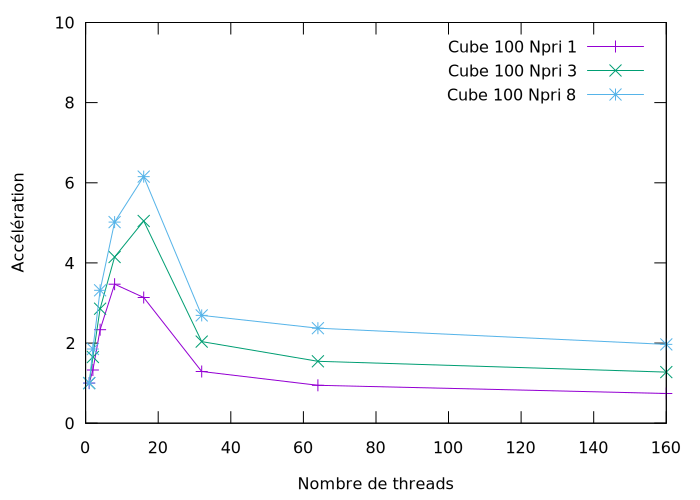
\includegraphics[width=0.49\textwidth]{res_trsv_ft_manu}
        }%
    \end{center}
    \caption{Performances sur Manumanu en utilisant une politique d'allocation first touch.}
\end{figure}
